%% This classfile tries to implement the lay-out of the beamer style beamerthemekuleuven2. This .sty-file can be downloaded here: https://www.kuleuven.be/communicatie/marketing/templates/presentatiemateriaal/index.html Not all options of the style are implemented in this class, for its purpose is merely to mimic the lay-out, and to provide a way to change the lay-out of presentations that were made using the "old" kulakbeamer class. For new documents, we recommend using the .sty-file instead.

\documentclass
   [kulak] % options: kul or kulak (default), handout 
   {kulakbeamer}

\usepackage[dutch]{babel}
\usepackage[utf8]{inputenc}
\usepackage[T1]{fontenc}

\title[Smart City]{Smart City}
\subtitle{Teamopdracht}
\author[Groep 6]{Groep 6}%eventueel nog aanpassen met onze namen 
\institute[Kulak]{KU Leuven Kulak}
\date{Academiejaar 2020 -- 2021}

%% Overview at begin of each section; delete if unwanted.

\AtBeginSection[]{
	\begin{frame}
	\frametitle{Overzicht} %Change to "Outline" for English presentation
	{
		\hypersetup{hidelinks} %disable link colors
		\hfill	{\large\parbox{.95\textwidth}{\tableofcontents[currentsection,hideothersubsections]}}
	}
\end{frame}}

\begin{document}

\begin{titleframe}
\titlepage
\end{titleframe}

\begin{outlineframe}[Overzicht]
\tableofcontents
\end{outlineframe}

 % % % Here you go  % % % 

\section{Inleiding}

\begin{frame}
\frametitle{Inleiding}
\begin{itemize}
	\item Wie: $1^{ste}$ jaar bachelorstudenten ingenieurswetenschappen
	\item Waarom: Vak Probleem oplossen en ontwerpen
	\item Wat: Zelfrijdend autootje met principe Smart City
	\item Gekozen optie: Richtingsaanwijzers

	\begin{block}{Definitie: Smart City}
		Een stad waarbij informatietechnologie gebruikt wordt om de stad te beheren en te besturen. \cite{SmartCity}
	\end{block}
\end{itemize}
\end{frame}


\section[Opdracht]{Opdracht}% eventueel aanpassen

\begin{frame}
\frametitle{De V's van vereisten}
\begin{itemize}
	\item Volglijnen, stoplijnen en verkeerslichten interpreteren
	\item Voorgaande wagen detecteren en botsing voorkomen
	\item Voldoende grote snelheid
	\item Vanop afstand kunnen ingrijpen
\end{itemize}

\end{frame}



\section{Aanpak}


\subsection{Planning}
\begin{frame}
	\frametitle{Planning}
	\begin{itemize}
		\item Onderdelen vergelijken
		\begin{itemize}
			\item Budget in rekening houden
			\item Stuklijst
		\end{itemize}
		\item Technisch
		\begin{itemize}
			\item 3D-modellen
			\item Technische tekeningen
		\end{itemize}
		\item Praktisch
		\begin{itemize}
			\item Assemblage
			\item Testen
			\item Implementatie
		\end{itemize}
	\end{itemize}
	
\end{frame}

\subsection{Onderdelen}

\begin{frame}
	\frametitle{Microcontroller \& chassis}
	\begin{columns}
		\column{.5\textwidth}
		\begin{figure}
			\centering
			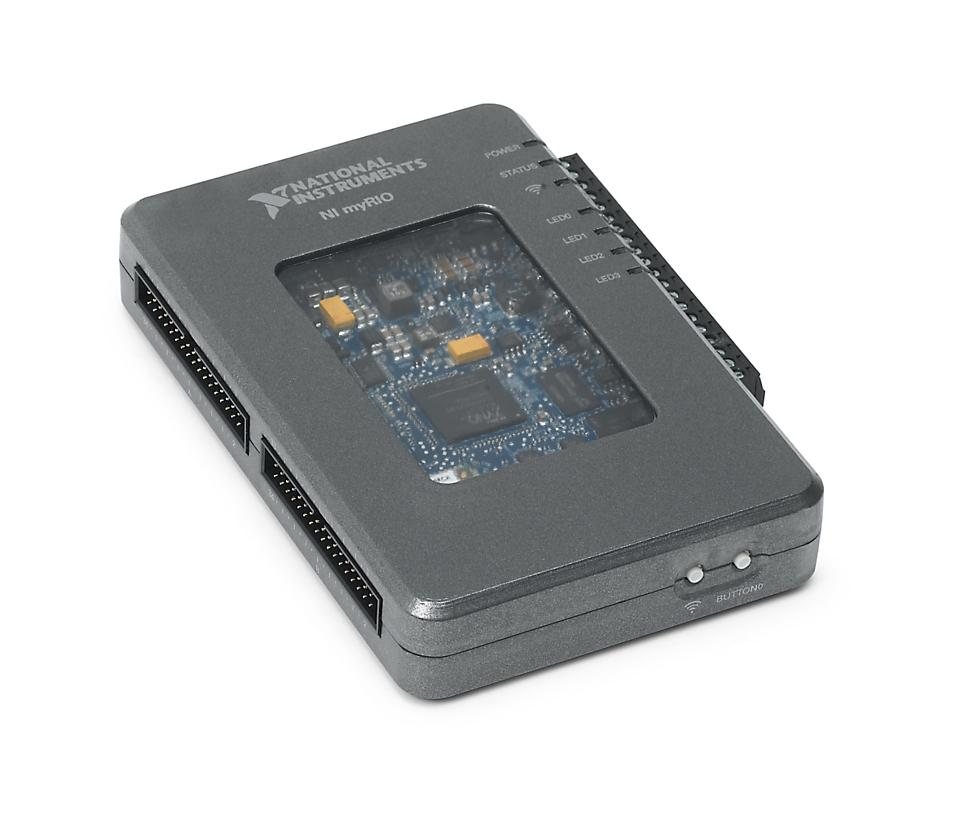
\includegraphics[width=.7\textwidth]{NI-myrio}
		\caption{NI MyRio}%nog te verwijzen
		\end{figure}
		\column{.5\textwidth}
		\begin{figure}
			\centering
			
\includegraphics[width=.45\textwidth]{chassis}
			\caption{Chassis}\cite{RobotChassisRechthoekigZwart}
		\end{figure}
		
	\end{columns}
	
\end{frame}

\begin{frame}
	\frametitle{Wielen \& ball caster}
	\begin{columns}
		\column{.5\textwidth}
		\begin{figure}
			\centering
			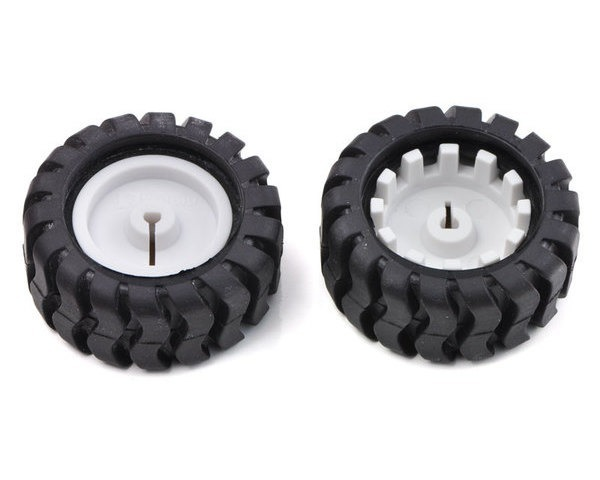
\includegraphics[width=.7\textwidth]{wielen}
			\caption{Wiel 42x19mm}\cite{Wiel42x19mm}
		\end{figure}
		\column{.5\textwidth}
		\begin{figure}
			\centering
			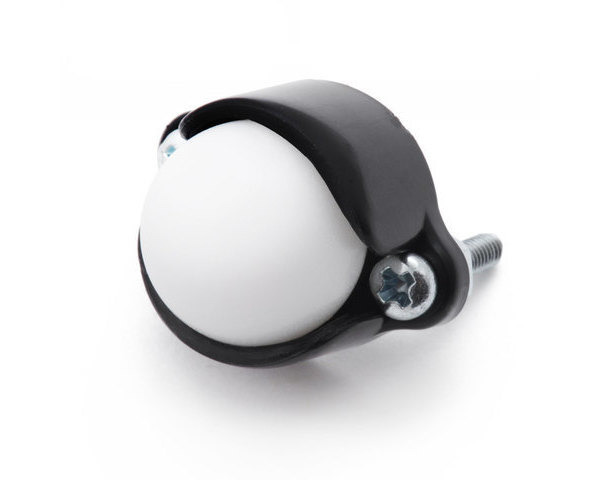
\includegraphics[width=.7\textwidth]{ballcaster}
			\caption{Ball Caster}\cite{BallCaster}
		\end{figure}
	\end{columns}
	
\end{frame}

\begin{frame}
	\frametitle{Sensoren}
	\begin{columns}
		\column{.3\textwidth}
		\begin{figure}
			\centering
			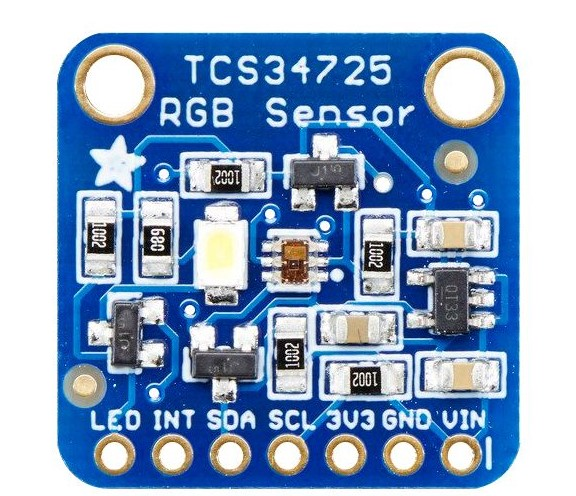
\includegraphics[width=.7\textwidth]{kleurensensor}
			\caption{Kleurensensor}\cite{TCS34725KleurSensorBOB}
		\end{figure}
		\column{.3\textwidth}
		\begin{figure}
			\centering
			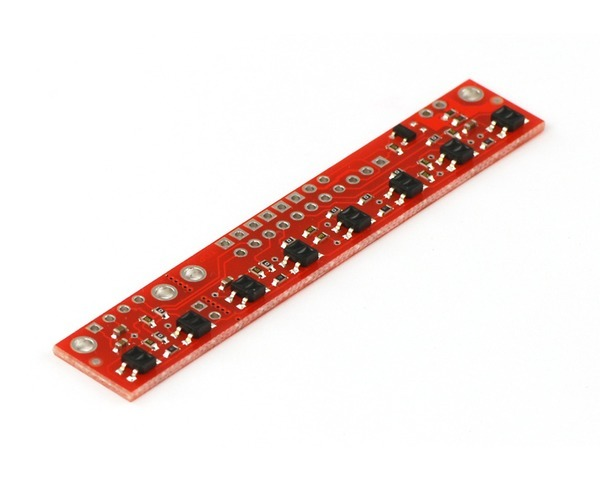
\includegraphics[width=.8\textwidth]{reflectiesensor}
			\caption{Analoge reflectiesensor}\cite{QTR-8AAnalogeReflexieSensorArray}
		\end{figure}
		\column{.3\textwidth}
		\begin{figure}
			\centering
			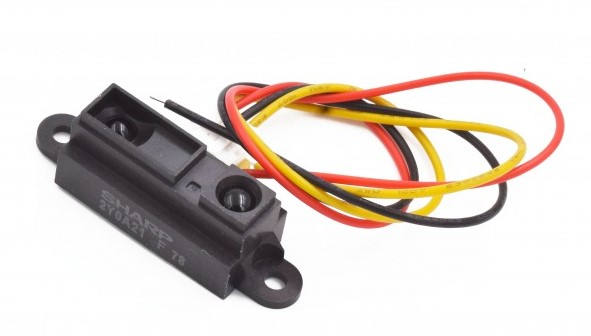
\includegraphics[width=.9\textwidth]{afstandssensor}
			\caption{Analoge afstandssensor}%nog te citeren
		\end{figure}
	\end{columns}
	
\end{frame}

\begin{frame}
	\frametitle{Gear Motor}
	\begin{columns}
		\column{.5\textwidth}
		\begin{figure}
			\centering
			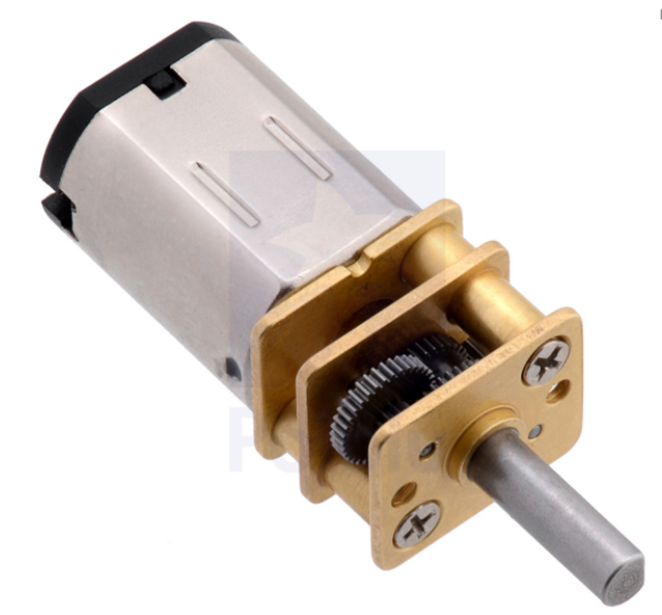
\includegraphics[width=.6\textwidth]{gear}
			\caption{Micro Metal Gear Motor 50:1 HP}\cite{MicroMetalGearMotor50:1HP}
		\end{figure}
		\column{.5\textwidth}
		\begin{figure}
			\centering
			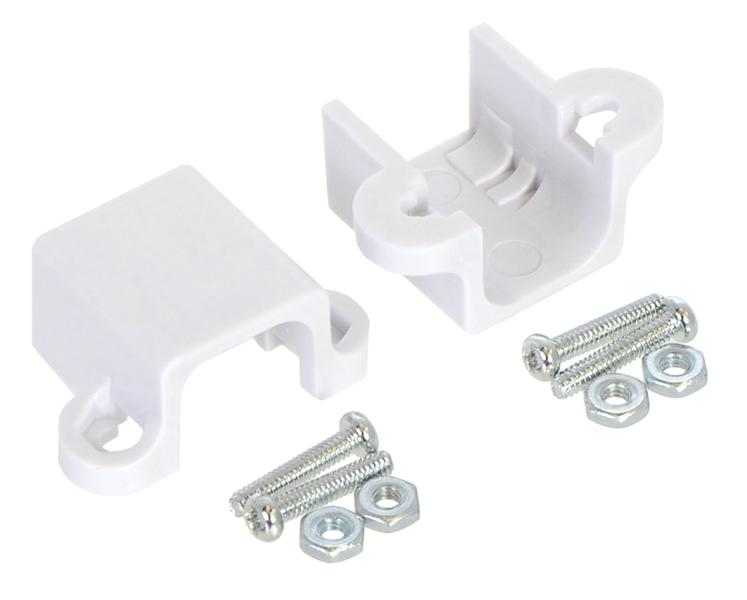
\includegraphics[width=.7\textwidth]{beugel}
			\caption{Motorbeugel}\cite{MicroMetalGearMotorBeugel}
		\end{figure}
	\end{columns}
	
\end{frame}



\subsection{Prijsbesteding}
\begin{frame}
	\frametitle{Prijsbesteding}
	\begin{itemize}
		\item Budget: 3500 eenheden
		\item Bieding: 1350 eenheden
		\item Uitgave aan onderdelen: 1615 eenheden
	\end{itemize}
\end{frame}



\section[Experimenten]{Experimenten met LabVIEW}

\begin{frame}
	\frametitle{Experimenten}
	\begin{itemize}
		\item Voorbeeldprogramma's voor sensoren
		\item Testen
		\begin{itemize}
			\item Reflectiesensor: witte bladzijde en zwart omhulsel laptop
			\item Afstandssensor: afstand object variëren
			\item nog aan te vullen
		\end{itemize}
	\end{itemize}.
\end{frame}



\section{Besluit}
\begin{frame}
\frametitle{Besluit}
Afsluitende tekst.
\end{frame}

\begin{frame}
\frametitle{Bronvermelding}
	\bibliographystyle{plain}
	\bibliography{bronnen_verslag}
	\bibliographystyle{unsrt}
\end{frame}

\end{document}
